\chapter{State of the Art}
\label{ch:sota}

This chapter reviews the technical foundations that support this project. It begins by exploring
the evolution of Artificial Intelligence (AI), tracing the shift from early symbolic AI based on
rules and logic techniques to modern sub-symbolic AI based on learning techniques. It then
introduces the core components of Deep Neural Networks (DNNs) that drive this sub-symbolic
paradigm, including feature extraction architectures, sequence and parallel processing
architectures, and attention mechanisms. Finally, the chapter contextualises these technologies by
reviewing previous work in Sign Language Recognition (SLR) and the main datasets used in American
Sign Language (ASL) research.

\section{From Symbolic to Subsymbolic AI}

Early AI systems were symbolic, representing knowledge through explicit logic and predefined rule
sets. They solved problems by applying human-authored rules, often organised as conditional
decision trees. While this paradigm flourished within constrained environments, it proved
inadequate for perception tasks, such as computer vision and speech, due to the inherent noise,
ambiguity, and high-dimensionality of real-world data. This phenomenon, termed the "knowledge
acquisition bottleneck", implies that as task complexity scales, the maintenance of handcrafted
rule bases becomes untenable.

In the context of sign language, symbolic approaches could encode basic gesture prototypes, but
they failed to capture the nuanced articulatory variation found across signers, camera angles and
execution speeds. A fixed rule for a hand shape may describe an idealised sign, yet the observed
motion in video changes with signer anatomy, partial occlusion, lighting and the temporal rhythm of
the execution. These sources of variation make exhaustive symbolic description impractical.

Subsymbolic AI addresses the same class of problems through statistical learning. Instead of
hard-coding expert rules for every possible case, a learning system estimates parameters from
examples. This transition was driven by advances in neural networks and statistical learning
theory, culminating in deep learning methods that learn hierarchical features directly from raw
inputs \cite{lecun2015deeplearning}. By treating perception as a high-dimensional optimisation
problem, these systems reduce the noise and ambiguity that previously led to the knowledge
acquisition bottleneck.

In the SLR domain, this transition mirrors the evolution of the field: moving away from attempts to
define a perfect hand-shape rules and towards architectures that extract latent features from raw
video data. Consequently, the burden of feature engineering shifts from the human expert to the
learning algorithm, allowing for a more fluid and robust interpretation of manual dynamics that
aligns with the success seen in modern speech recognition and object detection frameworks.

\section{Deep Neural Networks}
\label{sec:dnn}

A Deep Neural Network (DNN) is a parameterised function composed of layered computational
structures designed to map inputs to specific outputs. Each layer receives an input vector, applies
a linear transformation and passes the result through a non-linear activation function. A DNN
stacks several such layers sequentially, allowing the model to compose simple, low-level
mathematical transformations into progressively more abstract, high-level representations.
Figure~\ref{fig:dnn_basic} shows this structure as a mapping from input features to an output
prediction through hidden layers.

\begin{figure}[H]
    \centering
    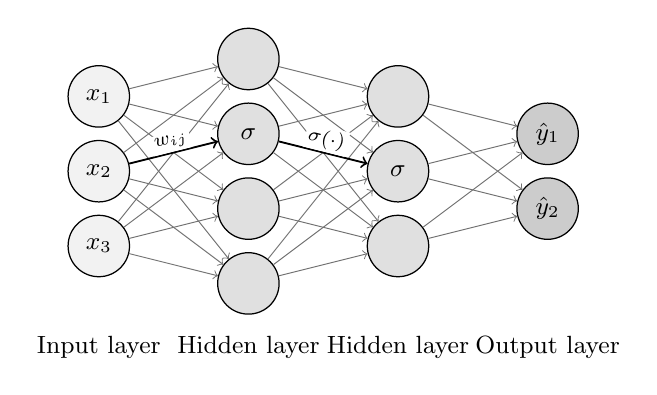
\begin{tikzpicture}[
            scale=0.95,
            every node/.style={font=\small},
            neuron/.style={draw=black,circle,minimum size=0.78cm,inner sep=0pt,line width=0.45pt},
            input neuron/.style={neuron,fill=black!5},
            hidden neuron/.style={neuron,fill=black!12},
            output neuron/.style={neuron,fill=black!20},
            connection/.style={->,black!55,line width=0.35pt},
            highlighted connection/.style={->,black,line width=0.65pt}
        ]
        \node[input neuron] (i1) at (0,2) {$x_1$};
        \node[input neuron] (i2) at (0,1) {$x_2$};
        \node[input neuron] (i3) at (0,0) {$x_3$};
        \node[hidden neuron] (h11) at (2,2.5) {};
        \node[hidden neuron] (h12) at (2,1.5) {$\sigma$};
        \node[hidden neuron] (h13) at (2,0.5) {};
        \node[hidden neuron] (h14) at (2,-0.5) {};
        \node[hidden neuron] (h21) at (4,2) {};
        \node[hidden neuron] (h22) at (4,1) {$\sigma$};
        \node[hidden neuron] (h23) at (4,0) {};
        \node[output neuron] (o1) at (6,1.5) {$\hat{y}_1$};
        \node[output neuron] (o2) at (6,0.5) {$\hat{y}_2$};

        \foreach \i in {i1,i2,i3}
        \foreach \h in {h11,h12,h13,h14}
        \draw[connection] (\i) -- (\h);
        \foreach \h in {h11,h12,h13,h14}
        \foreach \g in {h21,h22,h23}
        \draw[connection] (\h) -- (\g);
        \foreach \g in {h21,h22,h23}
        \foreach \o in {o1,o2}
        \draw[connection] (\g) -- (\o);

        \draw[highlighted connection] (i2) -- node[above,sloped,font=\scriptsize,fill=white,inner sep=1pt] {$w_{ij}$} (h12);
        \draw[highlighted connection] (h12) -- node[above,sloped,font=\scriptsize,fill=white,inner sep=1pt] {$\sigma(\cdot)$} (h22);

        \node at (0,-1.35) {Input layer};
        \node at (2,-1.35) {Hidden layer};
        \node at (4,-1.35) {Hidden layer};
        \node at (6,-1.35) {Output layer};
    \end{tikzpicture}
    \caption{Basic DNN structure. Inputs are transformed through hidden layers into an output prediction. Source: self-created.}
    \label{fig:dnn_basic}
\end{figure}

For a layer $l$, the computation can be written as:
\begin{equation}
    \mathbf{h}^{(l)} = \sigma\left(\mathbf{W}^{(l)}\mathbf{h}^{(l-1)} + \mathbf{b}^{(l)}\right)
\end{equation}
where $\mathbf{W}^{(l)}$ contains the learned weights, $\mathbf{b}^{(l)}$ is the bias vector and
$\sigma$ is the activation function. The Rectified Linear Unit (ReLU), defined as
$\text{ReLU}(x)=\max(0,x)$, is a common activation because it introduces non-linearity while keeping
the computation simple. The output layer depends on the task: classification layers estimate class
probabilities, whereas regression layers estimate continuous quantities such as coordinates.

Training adjusts the parameters $\theta=\{\mathbf{W},\mathbf{b}\}$ so that the function
$f_{\theta}$ maps inputs to the desired targets. The model computes a prediction, compares it with
the ground truth through a loss function and updates the parameters by gradient-based optimisation.
In this sense, a DNN is not a list of explicit rules but an optimised function approximator.

This formulation explains the link between DNNs and feature extraction. Intermediate layers do not
only transform the data numerically; they also produce representations that make the target task
easier. In Computer Vision, these representations may correspond to edges, textures, object parts
or pose coordinates. Feature extraction therefore denotes the process of converting raw
observations into informative variables that a later classifier or sequence model can use.

\section{Feature Extraction Architectures}
\label{sec:feature_extraction_architectures}

Feature extraction architectures convert video frames into representations that preserve relevant
visual information while reducing irrelevant variation. In SLR, two families are especially
important. Pixel-based techniques operate directly on image tensors, where each pixel stores colour
or intensity values. Pose estimation techniques first detect anatomical points and then represent
the signer through coordinates. The distinction matters because it determines whether the model
learns from appearance information or from a geometric abstraction of the body and hands.

\subsection{Pixel-Based Techniques}

A digital image can be represented as a tensor $\mathbf{x}\in\mathbb{R}^{H\times W\times C}$, where
$H$ and $W$ are height and width and $C$ is the number of colour channels, as shown in
Figure~\ref{fig:rgb_tensor_decomposition}. Pixel-based techniques use this tensor as the direct
input to the model. This preserves all visual information, including hand texture, background,
illumination and camera artefacts.

\begin{figure}[H]
    \centering
    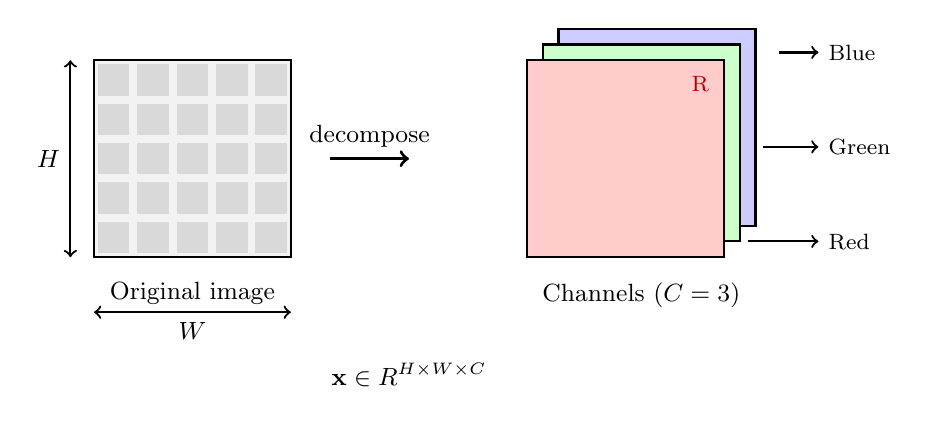
\begin{tikzpicture}[scale=1.0, every node/.style={font=\small}]
        % Original image (left)
        \begin{scope}[shift={(0,0)}]
            \draw[thick, fill=gray!10] (0,0) rectangle (2.5,2.5);
            % Simulate image content with a simple grid pattern
            \foreach \x in {0.25,0.75,1.25,1.75,2.25} {
                    \foreach \y in {0.25,0.75,1.25,1.75,2.25} {
                            \fill[gray!30] (\x-0.2,\y-0.2) rectangle (\x+0.2,\y+0.2);
                        }
                }
            \node[below] at (1.25,-0.2) {Original image};
            \draw[<->, thick] (-0.3,0) -- (-0.3,2.5) node[midway, left] {$H$};
            \draw[<->, thick] (0,-0.7) -- (2.5,-0.7) node[midway, below] {$W$};
        \end{scope}

        % Arrow
        \draw[->, very thick] (3.0,1.25) -- (4.0,1.25) node[midway, above] {decompose};

        % Three stacked channels (right)
        \begin{scope}[shift={(5.5,0)}]
            % Blue channel (back)
            \draw[thick, fill=blue!20] (0.4,0.4) rectangle (2.9,2.9);
            \node[blue!60!black] at (2.6,2.6) {\footnotesize B};
            % Green channel (middle)
            \draw[thick, fill=green!20] (0.2,0.2) rectangle (2.7,2.7);
            \node[green!60!black] at (2.4,2.4) {\footnotesize G};
            % Red channel (front)
            \draw[thick, fill=red!20] (0,0) rectangle (2.5,2.5);
            \node[red!70!black] at (2.2,2.2) {\footnotesize R};

            \node[below] at (1.45,-0.2) {Channels ($C=3$)};

            % Annotations
            \draw[->, thick] (3.2,2.6) -- (3.7,2.6) node[right] {\footnotesize Blue};
            \draw[->, thick] (3.0,1.4) -- (3.7,1.4) node[right] {\footnotesize Green};
            \draw[->, thick] (2.8,0.2) -- (3.7,0.2) node[right] {\footnotesize Red};
        \end{scope}

        % Tensor notation below
        \node at (4.0,-1.5) {$\mathbf{x} \in \mathbb{R}^{H \times W \times C}$};
    \end{tikzpicture}
    \caption[Decomposition of a digital RGB image into its three colour channels.]{Decomposition of a digital RGB image into its three colour channels. The image is represented as a tensor $\mathbf{x} \in \mathbb{R}^{H \times W \times C}$, where $H$ and $W$ are the spatial dimensions and $C = 3$ corresponds to the red, green and blue channels.\textsuperscript{1}}
    \label{fig:rgb_tensor_decomposition}
    \vspace{0.3em}
    \begin{minipage}{0.92\textwidth}
        \footnotesize\textsuperscript{1} Figure source code generated by OpenAI GPT-5.5 in High mode, OpenAI, May 20, 2026, from a prompt asking for a diagram representing a digital image as a tensor $\mathbf{x} \in \mathbb{R}^{H \times W \times C}$ and decomposing it into its RGB colour channels.
    \end{minipage}
\end{figure}

Convolutional Neural Networks (CNNs) are the standard DNN architecture for pixel-based computer
vision \cite{lecun2015deeplearning}. CNN architectures stack convolutional, activation and pooling
layers. A convolutional layer applies a small matrix of learned parameters, called a kernel or
filter, across local regions of the image. At each spatial position, the kernel computes a response
that indicates whether a visual pattern is present. The collection of responses produced by one
kernel is a feature map.

For input tensor $\mathbf{x}$ and output feature map $\mathbf{y}$, a convolutional layer can be
written as:
\begin{equation}
    \mathbf{y}_{i,j,k} =
    \sigma\left(
    \sum_{c=1}^{C} \sum_{u,v} \mathbf{w}_{u,v,c,k}\mathbf{x}_{i+u,j+v,c} + b_k
    \right)
\end{equation}
where $\mathbf{w}$ is the set of kernels, $b_k$ is the bias for feature map $k$ and $\sigma$ is the
activation function. Because the same kernel is reused across the image, convolutional layers encode
translation equivariance: if a pattern shifts in the image, its corresponding activation shifts in
the feature map.

Pooling layers reduce the spatial resolution of feature maps by summarising local neighbourhoods,
commonly through maximum or average values. This supports local translation invariance, since small
shifts in the input produce similar pooled activations. Early layers usually respond to oriented
edges and simple textures; deeper layers combine those responses into larger shapes and
object-level cues, as illustrated in Figure~\ref{fig:cnn_features}. AlexNet
\cite{krizhevsky2012imagenet} and ResNet \cite{he2016resnet} are established examples of this
hierarchical design.

\begin{figure}[H]
    \centering
    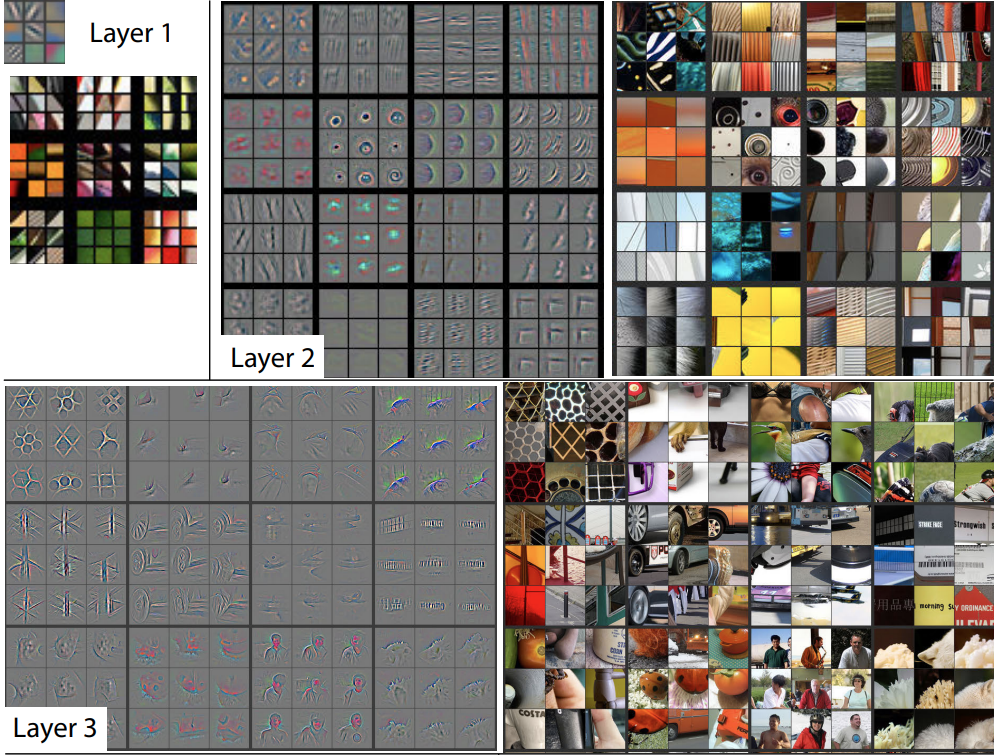
\includegraphics[width=1.0\textwidth]{images/zeiler_fergus_features.png}
    \caption{Hierarchical feature representations learned by a CNN.
        Layer 1 responds to oriented edges and simple colour gradients;
        Layer 2 captures corners, circular patterns and basic textures;
        Layer 3 represents more complex textures and object parts.
        Adapted from Zeiler and Fergus \cite{zeiler2014visualizing}.}
    \label{fig:cnn_features}
\end{figure}

Figure~\ref{fig:cnn_arch} shows the AlexNet architecture. The diagram is relevant here because it
illustrates the repeated pattern of convolution, pooling and fully connected layers that made deep
pixel-based recognition practical.

\begin{figure}[H]
    \centering
    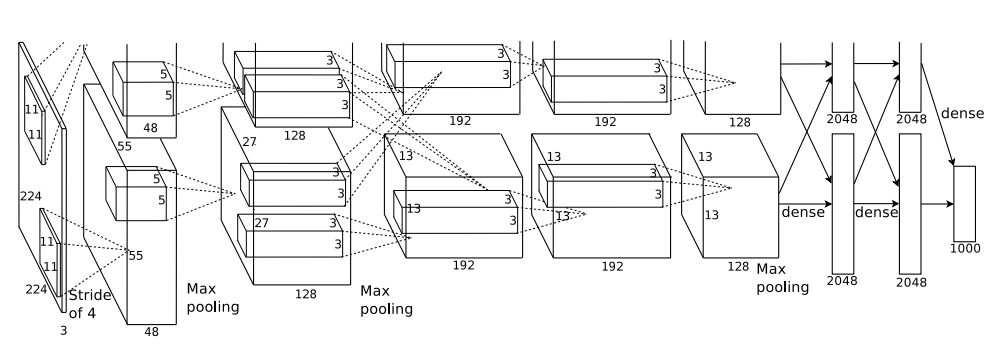
\includegraphics[width=0.9\textwidth]{images/alexnet_architecture.png}
    \caption{AlexNet architecture, showing stacked convolutional and pooling layers followed by fully connected layers. Source: Krizhevsky et al. \cite{krizhevsky2012imagenet}.}
    \label{fig:cnn_arch}
\end{figure}

In SLR context, pixel-based CNNs can learn discriminative visual patterns directly from raw video
frames. However, their main limitation is that they also receive information that may not define
the sign, including background, skin tone and recording conditions. When the available dataset is
limited, this can encourage the model to fit appearance correlations instead of sign structure.

\subsection{Pose Estimation Techniques}

Pose estimation involves predicting the spatial coordinates of anatomical points (landmarks) within
an image or video frame, which constitutes a regression task because it requires calculating
continuous numerical values rather than selecting a distinct class from a fixed set. In hand pose
estimation, many landmarks correspond to joints, which are anatomical articulations such as
knuckles, while fingertip landmarks mark the end of each finger. A regression-based pose estimator
therefore predicts landmark coordinates rather than a discrete class label.

Figure~\ref{fig:mediapipe_landmark_example} shows an example of the type of hand skeleton produced
by a landmark-based hand tracking system. The image illustrates how the visual hand region is
converted into a set of keypoints connected according to the anatomical structure of the hand.

\begin{figure}[H]
    \centering
    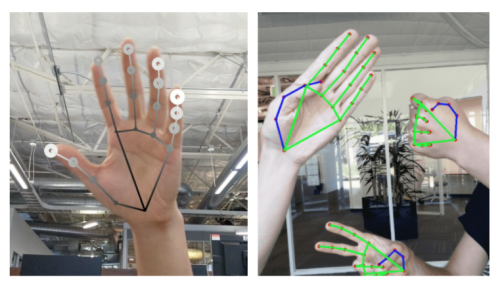
\includegraphics[width=0.65\textwidth]{images/landmark_image_paper.png}
    \caption{Rendered hand tracking result with hand landmarks and multi-hand tracking output. Source: Zhang et al. \cite{zhang2020mediapipehands}.}
    \label{fig:mediapipe_landmark_example}
\end{figure}

Pose pipelines are commonly organised as top-down or bottom-up systems. A top-down pipeline first
detects the relevant object or body part, then estimates landmarks inside the detected region. A
bottom-up pipeline first predicts candidate landmarks across the image, then groups them into
instances. Both approaches convert raw image evidence into a structured geometric representation.

MediaPipe Hands \cite{zhang2020mediapipehands} is a widely used hand pose estimation system. It
uses the top-down structure shown in Figure~\ref{fig:mediapipe_pipeline}: a hand detector proposes
a region of interest, and a landmark model estimates hand coordinates inside that cropped region.

\begin{figure}[H]
    \centering
    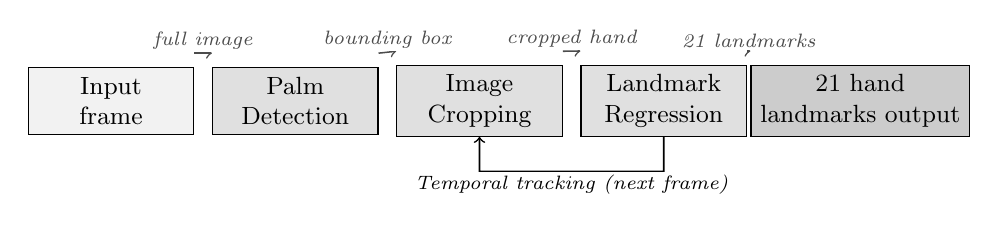
\begin{tikzpicture}[
            scale=0.78,
            every node/.style={font=\small},
            stage/.style={draw=black,rectangle,minimum width=2.10cm,minimum height=0.85cm,align=center,line width=0.45pt},
            input stage/.style={stage,fill=black!5},
            process stage/.style={stage,fill=black!12},
            output stage/.style={stage,fill=black!20,minimum width=2.45cm},
            flow/.style={->,black!70,line width=0.55pt},
            tracking/.style={->,black,line width=0.6pt}
        ]
        \node[input stage] (input) at (0,0) {Input\\frame};
        \node[process stage] (palm) at (3.00,0) {Palm\\Detection};
        \node[process stage] (crop) at (6.00,0) {Image\\Cropping};
        \node[process stage] (regress) at (9.00,0) {Landmark\\Regression};
        \node[output stage] (output) at (12.20,0) {21 hand\\landmarks output};

        \draw[flow] ([yshift=0.22cm]input.north east) --
        node[above,font=\scriptsize\itshape,fill=white,inner sep=1pt] {full image}
        ([yshift=0.22cm]palm.north west);
        \draw[flow] ([yshift=0.22cm]palm.north east) --
        node[above,font=\scriptsize\itshape,fill=white,inner sep=1pt] {bounding box}
        ([yshift=0.22cm]crop.north west);
        \draw[flow] ([yshift=0.22cm]crop.north east) --
        node[above,font=\scriptsize\itshape,fill=white,inner sep=1pt] {cropped hand}
        ([yshift=0.22cm]regress.north west);
        \draw[flow] ([yshift=0.22cm]regress.north east) --
        node[above,font=\scriptsize\itshape,fill=white,inner sep=1pt] {21 landmarks}
        ([yshift=0.22cm]output.north west);

        \draw[tracking]
        (regress.south) -- (9.00,-1.15) --
        node[below,font=\scriptsize\itshape,fill=white,inner sep=1pt] {Temporal tracking (next frame)}
        (6.00,-1.15) -- (crop.south);
    \end{tikzpicture}
    \caption{MediaPipe Hands pipeline. The palm detector locates the hand region on the first frame or when tracking is lost; the landmark model then regresses 21 three-dimensional landmarks inside the cropped region. Subsequent frames reuse the landmarks from the previous frame, avoiding running palm detection on every frame. Source: self-created, adapted from Zhang et al. \cite{zhang2020mediapipehands}.}
    \label{fig:mediapipe_pipeline}
\end{figure}

The process consists of the following stages:
\begin{enumerate}
    \item \textbf{Palm detection:} The full image frame is processed by a single-shot detector, which
          estimates a bounding region around the palm and defines the hand region of interest.
    \item \textbf{Image cropping:} The detected region is cropped and aligned around the hand,
          producing a normalised hand image for the landmark model.
    \item \textbf{Landmark regression:} The landmark model receives the cropped hand image and
          regresses the coordinates of 21 three-dimensional hand landmarks.
    \item \textbf{Temporal tracking:} When the hand remains visible, the pipeline reuses landmarks and
          region-of-interest information from the previous frame to obtain a continuous landmark
          sequence.
\end{enumerate}

For SLR, landmark sequences provide a compact description of hand shape and movement. They remove
much of the raw appearance signal and make it possible to derive additional geometric features such
as bone vectors, joint angles and distances between fingers. The cost of this abstraction is that
pose estimators may fail under occlusion, motion blur or unusual camera angles, and hand-only
landmarks omit non-manual cues such as facial expression and upper-body movement.

\section{Sequence Processing Architectures}
\label{sec:sequence_processing_architectures}

Isolated sign recognition is a temporal classification problem. This means that the input is not a
single image but an ordered sequence of feature vectors, one per frame or sampled time step. A
sequence processing layer therefore receives $\{\mathbf{x}_1,\mathbf{x}_2,\ldots,\mathbf{x}_T\}$
and produces a representation that accounts for temporal order.

\subsection{Recurrent Layers}

Recurrent Neural Networks (RNNs) process a sequence by maintaining a hidden state. At time $t$, the
layer combines the current input $\mathbf{x}_t$ with the previous hidden state $\mathbf{h}_{t-1}$:
\begin{equation}
    \mathbf{h}_t =
    \phi(\mathbf{W}_{xh}\mathbf{x}_t + \mathbf{W}_{hh}\mathbf{h}_{t-1} + \mathbf{b}_h)
\end{equation}
where $\phi$ is an activation function. The same parameters are shared at every time step, as shown
in Figure~\ref{fig:rnn_unrolled}. This sharing lets the layer process sequences of different
lengths while applying the same transition rule throughout the video.

\begin{figure}[H]
    \centering
    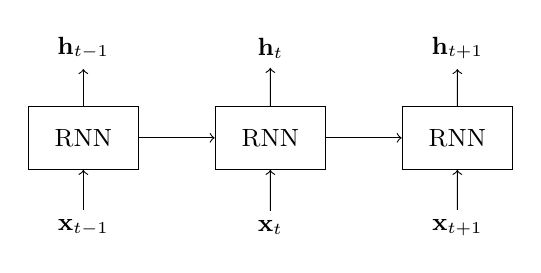
\begin{tikzpicture}[scale=0.95, every node/.style={font=\small}]
        \node[draw,minimum width=1.4cm,minimum height=0.8cm] (r1) at (0,0) {RNN};
        \node[draw,minimum width=1.4cm,minimum height=0.8cm] (r2) at (2.5,0) {RNN};
        \node[draw,minimum width=1.4cm,minimum height=0.8cm] (r3) at (5,0) {RNN};
        \node (x1) at (0,-1.2) {$\mathbf{x}_{t-1}$};
        \node (x2) at (2.5,-1.2) {$\mathbf{x}_{t}$};
        \node (x3) at (5,-1.2) {$\mathbf{x}_{t+1}$};
        \node (y1) at (0,1.2) {$\mathbf{h}_{t-1}$};
        \node (y2) at (2.5,1.2) {$\mathbf{h}_{t}$};
        \node (y3) at (5,1.2) {$\mathbf{h}_{t+1}$};
        \draw[->] (x1) -- (r1);
        \draw[->] (x2) -- (r2);
        \draw[->] (x3) -- (r3);
        \draw[->] (r1) -- (y1);
        \draw[->] (r2) -- (y2);
        \draw[->] (r3) -- (y3);
        \draw[->] (r1) -- (r2);
        \draw[->] (r2) -- (r3);
    \end{tikzpicture}
    \caption{Unrolled recurrent layer. The same recurrent computation is applied at each time step while the hidden state carries information forward. Source: self-created.}
    \label{fig:rnn_unrolled}
\end{figure}

Training recurrent layers uses Backpropagation Through Time (BPTT) \cite{werbos1990bptt}, which
unfolds the recurrent computation across the sequence and propagates the loss backwards through the
unfolded graph. As the number of time steps increases, standard recurrent layers frequently
encounter the vanishing gradient problem \cite{bengio1994longterm}. The gradient signal becomes too
small to preserve information from early time steps, which limits long-range temporal modelling.

The recurrent layer described above represents the baseline architecture. To address its
operational limitations, more sophisticated gated variants have been developed:
\begin{itemize}
    \item Long Short-Term Memory (LSTM) layers, which introduce a cell state and gates to regulate
          information flow.
    \item Gated Recurrent Unit (GRU) layers, which simplify the LSTM design while retaining gated
          memory.
\end{itemize}

\subsection{Long Short-Term Memory Layers}

Long Short-Term Memory (LSTM) layers were proposed by Hochreiter and Schmidhuber
\cite{hochreiter1997lstm} to improve the modelling of long temporal dependencies. An LSTM layer
maintains two vectors: the hidden state $\mathbf{h}_t$, which is exposed to the next layer or
output, and the cell state $\mathbf{C}_t$, which carries memory along the sequence.

The LSTM cell regulates this memory through gates. The forget gate controls which information is
removed from the cell state, the input gate controls which new information is written and the
output gate controls which part of the cell state becomes the hidden state.
Figure~\ref{fig:rnn_comparison} (a) represents these gates as $f$, $i$ and $o$, and shows how the
cell state $C$ provides a direct path for information flow.

This gated memory path is the mechanism referred to as the Constant Error Carousel. It reduces the
decay of the error signal during BPTT and allows the layer to retain information over longer time
spans than a simple recurrent layer. The cost is computational: each time step requires several
linear transformations, increasing both parameter count and training time.

\subsection{Gated Recurrent Unit Layers}

Gated Recurrent Unit (GRU) layers were introduced by Chung et al. \cite{chung2014gru} as a simpler
gated recurrent alternative. A GRU layer removes the separate cell state and stores memory directly
in the hidden state $\mathbf{h}_t$. It uses two gates, shown in Figure~\ref{fig:rnn_comparison}(b):
the update gate $z$ and the reset gate $r$.

\begin{figure}[H]
    \centering
    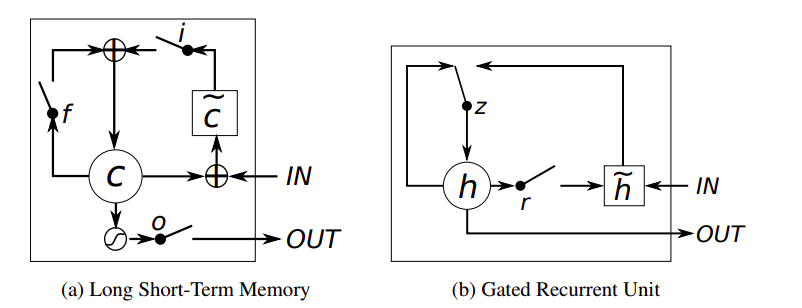
\includegraphics[width=0.8\textwidth]{images/gru_paper_diagram.png}
    \caption{Comparison of gated recurrent units. (a) LSTM cell with input, forget and output gates. (b) GRU cell with update and reset gates. Source: Chung et al. \cite{chung2014gru}.}
    \label{fig:rnn_comparison}
\end{figure}

The GRU gate equations at time $t$ are:
\begin{align}
    \mathbf{z}_t & = \sigma(\mathbf{W}_z\mathbf{x}_t + \mathbf{U}_z\mathbf{h}_{t-1} + \mathbf{b}_z) \\
    \mathbf{r}_t & = \sigma(\mathbf{W}_r\mathbf{x}_t + \mathbf{U}_r\mathbf{h}_{t-1} + \mathbf{b}_r)
\end{align}
The reset gate controls how much previous information is used to compute the candidate hidden state
$\tilde{\mathbf{h}}_t$. The update gate controls the interpolation between the previous hidden
state and the candidate state:
\begin{equation}
    \mathbf{h}_t = (1-\mathbf{z}_t)\odot\mathbf{h}_{t-1} + \mathbf{z}_t\odot\tilde{\mathbf{h}}_t
\end{equation}
When $\mathbf{z}_t$ is close to zero, the layer copies most of the previous hidden state. When it is
close to one, the layer replaces it with new information. This gives GRU layers a compact mechanism
for modelling temporal dependencies with fewer parameters than LSTM layers.

\section{Attention Mechanisms}
\label{sec:attention_mechanisms}

Attention mechanisms assign different weights to different parts of an input sequence. In neural
machine translation, Bahdanau et al. \cite{bahdanau2014neural} introduced attention to avoid
compressing a full source sentence into a single fixed-length vector. The same idea applies to
video recognition: not every frame contributes equally to the final prediction.

Given encoder states $\{\mathbf{h}_t\}_{t=1}^T$, an attention module computes a score $e_t$ for
each time step and normalises the scores with a softmax function:
\begin{equation}
    \alpha_t = \frac{\exp(e_t)}{\sum_{k=1}^{T}\exp(e_k)}, \quad e_t = a(\mathbf{s}, \mathbf{h}_t)
\end{equation}
where $a(\cdot)$ is a scoring function and $\alpha_t$ is the attention weight assigned to time step
$t$. The context vector is then computed as:
\begin{equation}
    \mathbf{c} = \sum_{t=1}^{T}\alpha_t\mathbf{h}_t
\end{equation}
Figure~\ref{fig:attention_mech} shows this weighted combination: the decoder state attends to
encoder annotations through weights $\alpha_{t,1},\alpha_{t,2},\ldots,\alpha_{t,T}$.

\begin{figure}[H]
    \centering
    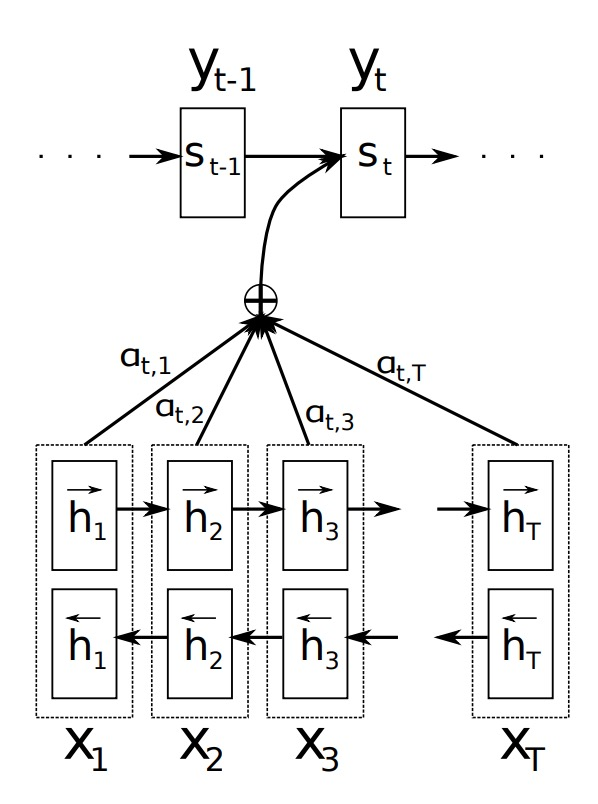
\includegraphics[width=0.5\textwidth]{images/temporal_attention.png}
    \caption{Attention mechanism in an encoder-decoder architecture. The context vector is a weighted sum of encoder annotations. Source: Bahdanau et al. \cite{bahdanau2014neural}.}
    \label{fig:attention_mech}
\end{figure}

For example, in an SLR clip of the sign \textit{drink}, the first frames may show the hand moving
towards the mouth, the central frames may contain the class-defining motion and the final frames
may show the hand returning to rest. Temporal attention can assign higher weights to the central
frames and lower weights to the preparation and recovery frames. This does not remove the need for
a sequence model; it adds a learned weighting stage over the temporal representation produced by
that model.

\subsection{Transformer Layers}

Transformer layers extend the attention idea by making self-attention the main operation of the
sequence model \cite{vaswani2017attention}. Instead of updating a hidden state step by step, as in
a recurrent layer, self-attention compares every position in the sequence with every other
position. Each time step is projected into query, key and value vectors. The query-key similarities
determine which positions are most relevant to each other, and the value vectors are combined
according to those attention weights.

This formulation allows a Transformer to model relationships between distant frames without passing
information through all intermediate time steps. It also supports parallel computation across the
sequence, which is useful when large datasets and long inputs are available. However, because the
model does not process frames in their natural order by default, positional information must be
added so that the network can distinguish earlier frames from later ones.

In SLR, Transformer-based models are relevant because signs often contain dependencies between
non-adjacent moments of the motion. At the same time, they can be more data-demanding than
recurrent layers, especially in small word-level datasets. For this reason, Transformers are best
understood in this work as attention-based sequence models to compare against recurrent
alternatives, rather than as an automatic replacement for LSTM or GRU layers.

\section{Related Work in Sign Language Recognition}
\label{sec:related_slr_work}

SLR research can be organised according to the recognition setting and the type of visual
representation used by the model. Survey work distinguishes between isolated sign recognition,
continuous sign recognition and sign language translation \cite{koller2020signlanguage,
rastgoo2021signlanguage,bragg2019signlanguagerecognition}. Isolated recognition assigns a single
gloss to a trimmed clip, which is the scope of this project. Continuous recognition must segment
and classify signs from longer streams, while translation must produce spoken-language text and
account for grammar, context and non-manual markers.

\paragraph{Detection-based approaches:}
Earlier vision pipelines often treated hands as regions to be detected before classification.
Modern object detectors such as Faster Region-based Convolutional Neural Network (Faster R-CNN)
\cite{ren2015fasterrcnn}, Single Shot MultiBox Detector (SSD) \cite{liu2016ssd}, EfficientDet
\cite{tan2020efficientdet} and the You Only Look Once (YOLO) family
\cite{redmon2016yolo,redmon2018yolov3} frame this problem as locating objects and assigning class
scores in images. YOLO is especially relevant for real-time hand detection because it performs
detection in a single forward pass, and YOLOv8 is a current implementation frequently used in
practical detection pipelines \cite{jocher2023yolov8}.

\paragraph{Pixel-based deep learning approaches:}
With the adoption of DNNs, many SLR systems moved from handcrafted descriptors towards models that
learn visual features directly from video frames. Pixel-based CNNs extract frame-level appearance
patterns, while recurrent layers model their temporal evolution and attention modules weight the
most informative moments of the sequence. Transformer-based work such as Sign Language Transformers
\cite{camgoz2020signlanguagetransformers} and STMC-Transformer \cite{yin2020stmc} shows how
attention-based sequence models have been applied to continuous recognition and translation
settings.

\paragraph{Pose-based approaches:}
Pose-based methods replace raw frames with landmark sequences, reducing dimensionality and limiting
the influence of background appearance. Bohacek and Hruz \cite{bohacek2022spoter} proposed a
pose-based Transformer for word-level SLR, while Sign2Pose \cite{eunice2023sign2pose} combines pose
features and Transformer-based gloss prediction on WLASL. This project is situated in the
pose-based line: MediaPipe Hands provides hand landmarks, and the recognition model evaluates
recurrent and attention-based temporal processing.

\paragraph{Datasets and evaluation context:}
Word-level ASL recognition is strongly associated with WLASL and MS-ASL. Li et al.
\cite{li2020wlasl} introduced WLASL together with benchmark comparisons for word-level recognition
from video, while Joze and Koller \cite{joze2019msasl} introduced MS-ASL as a larger ASL benchmark.
Both works helped move isolated SLR evaluation away from small curated vocabularies and towards
larger, noisier video collections. Large-scale work such as BSL-1K \cite{albanie2020bsl1k} also
highlights that dataset scale, weak supervision and cross-dataset transfer remain central concerns
in sign recognition research.

\section{Dataset Limitations}
\label{sec:sota_datasets}

SLR systems depend strongly on the datasets available for training and evaluation. Unlike general
image recognition, sign language recognition still lacks abundant large-scale benchmarks across
languages, domains and signer populations. Dataset design therefore shapes what a recognition model
can learn: the vocabulary determines the classification space, recording conditions affect visual
variation and annotation practice defines the gloss labels used for evaluation.

The main limitations are fourfold. First, many sign datasets contain a limited number of examples
per class, which makes it difficult to train high-capacity temporal models without overfitting.
Second, class imbalance is common: frequent signs tend to have many more examples than rare signs,
so aggregate accuracy may hide poor behaviour on under-represented glosses. Third, clips collected
from online sources introduce uncontrolled variation in camera quality, viewpoint, signer
appearance, background, duration and execution style. Finally, dataset attrition can occur when
source videos are removed or made private, reducing reproducibility over time.

These limitations affect how experimental results should be interpreted. A model can perform well
on a constrained benchmark while still struggling to generalise to new signers, recording
conditions or larger vocabularies. Auxiliary resources such as static alphabet datasets or
hand-detection corpora are useful for engineering stages, but they should not be treated as
word-level SLR benchmarks because they do not evaluate temporal sign dynamics.